%\documentclass[dvipsnames,border=10pt,tikz]{standalone}
\documentclass[convert={density=300,size=1080x800,outext=.png}]{standalone}
\usepackage{tikz}
\usetikzlibrary{shapes.geometric}
\usepackage{xcolor}


\begin{document}

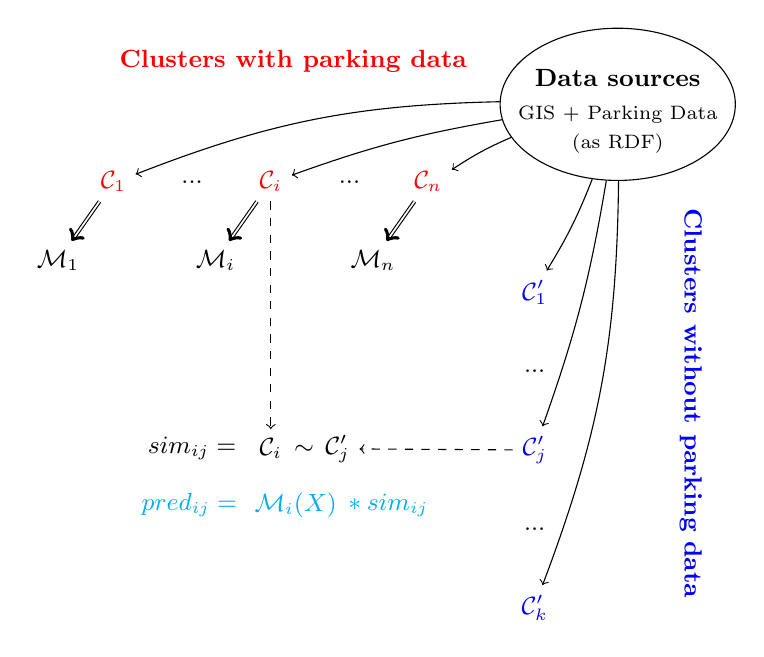
\begin{tikzpicture}
[
graph largevertex/.style={ellipse,draw,font=\small,minimum width = 85pt, minimum height=55pt},
graph smallvertex/.style={circle,draw,font=\small,minimum size = 5pt,inner sep=0pt},
graph rectangle/.style={rectangle,draw,font=\small,minimum width = 150pt, minimum height = 35pt},
graph smallrectangle/.style={rectangle,draw,font=\small,text=blue,minimum width = 10pt, minimum height = 10pt},
graph text/.style={font=\small},
graph redtext/.style={font=\small, color=red, },
graph bluetext/.style={font=\small, color=blue},
graph cyantext/.style={font=\small, color=cyan},
graph smalltext/.style={font=\scriptsize},
graph blueverticaltext/.style={font=\small, rotate=-90, color=blue}
]

% Cwith
\node[graph redtext] (C1) {$\mathcal{C}_1$};
\node[graph text, right of=C1] (C2) {$...$};
\node[graph redtext, right of=C2] (C3) {$\mathcal{C}_i$};
\node[graph text, right of=C3] (C4) {$...$};
\node[graph redtext, right of=C4] (C5) {$\mathcal{C}_n$};

% Cwout
\node[graph bluetext, right of=C5, yshift=-4em, xshift=1em] (C'1) {$\mathcal{C}'_1$};
\node[graph text, below of=C'1] (C'2) {$...$};
\node[graph bluetext, below of=C'2] (C'3) {$\mathcal{C}'_j$};
\node[graph text, below of=C'3] (C'4) {$...$};
\node[graph bluetext, below of=C'4] (C'5) {$\mathcal{C}'_k$};

% Models
\node[graph text, below of=C1, xshift=-2em] (M1) {$\mathcal{M}_1$};
%\node[graph text, below of=C2, xshift=-2em] (M2) {$...$};
\node[graph text, below of=C3, xshift=-2em] (M3) {$\mathcal{M}_i$};
%\node[graph text, below of=C4, xshift=-2em] (M4) {$...$};
\node[graph text, below of=C5, xshift=-2em] (M5) {$\mathcal{M}_n$};

\draw[double,->] (C1) -- (M1);
\draw[double,->] (C3) -- (M3);
\draw[double,->] (C5) -- (M5);

% center first row
\node[graph text, below of=C3, yshift=-6.8em] (D2) {$\mathcal{C}_i$};
\draw[dashed,->] (C3) -- (D2);
\node[graph text, left of=D2, xshift=0em] (D1) {$sim_{ij}=$};
\node[graph text, right of=D2, xshift=-1em] (D3) {$\sim\,\mathcal{C}'_j$};
\draw[dashed,->] (C'3) -- (D3);

% center second row
\node[graph cyantext, below of=M3, yshift=-6em, xshift=2.9em] (E2) {$\mathcal{M}_i(X)$};
%\draw[dashed,->] (M3) -- (E2);
\node[graph cyantext, right of=E2, xshift=0.5em] (E3) {$\ast\:    
 sim_{ij}$};
\node[graph cyantext, left of=E2, xshift=-1em] (E1) {$pred_{ij}=$};

% upper right graph
\node[graph largevertex, right of=C5, xshift=4em, yshift=2.8em] (S1) {};
%\node[graph smallvertex, above of=S1, xshift=0em, yshift=-1.8em] (S2) {};
%\node[graph smallvertex, below of=S2, xshift=-0.9em, yshift=0.9em] (S3) {};
%\node[graph smallvertex, below of=S2, xshift=0.9em, yshift=0.9em] (S4) {};
%\draw (S2) -- (S3);
%\draw (S2) -- (S4);
%\draw (S3) -- (S4);
\node[graph text, below of=S1, yshift=3.8em] (S2) {\textbf{Data sources}};
\node[graph smalltext, below of=S2, yshift=1.5em] (S3) {GIS + Parking Data};
\node[graph smalltext, below of=S3, yshift=1.8em] (S4) {(as RDF)};

% clustering arrows
\draw[->] (S1) to [bend right=10] (C1);
\draw[->] (S1) to [bend right=5] (C3);
\draw[->] (S1) to [bend right=5] (C5);
\draw[->] (S1) to [bend left=10] (C'5);
\draw[->] (S1) to [bend left=5] (C'3);
\draw[->] (S1) to [bend left=5] (C'1);

% rectangle Cwith
%\node[graph rectangle, above of=C3, xshift=0em, yshift=-1.6em] (R) {};
%\node[graph smallrectangle, above of=C1, xshift=-1.15em, yshift=-0.5em] (R) {$\textrm{P}$};

% upper band
\node[graph redtext, above of=C1, xshift=6.5em, yshift=1.5em] (F1) {\textbf{Clusters with parking data}};
%\node[graph text, below of=F1, xshift=0.5em, yshift=1.5em] (F2) {parking data};

% right-hand size band
\node[graph blueverticaltext, above of=C'1, xshift=4.0em, yshift=2.8em] (G1) {\textbf{Clusters without parking data}};

\end{tikzpicture}  

\end{document}